%%%%%%%%%%%%%%%%%%%%%%%%%%%%%%%%%%%%%%%%%
% BA04 presentation 
% LaTeX Template
% Version 1.0 (14/12/14)
%
% This template has been downloaded from:
% http://www.LaTeXTemplates.com
%
% License:
% CC BY-NC-SA 3.0 (http://creativecommons.org/licenses/by-nc-sa/3.0/)
%
%%%%%%%%%%%%%%%%%%%%%%%%%%%%%%%%%%%%%%%%%

%----------------------------------------------------------------------------------------
%	PACKAGES AND THEMES
%----------------------------------------------------------------------------------------

\documentclass{beamer}
\usepackage{etex}

\mode<presentation> {

% The Beamer class comes with a number of default slide themes
% which change the colors and layouts of slides. Below this is a list
% of all the themes, uncomment each in turn to see what they look like.

\usetheme{Berlin}

% As well as themes, the Beamer class has a number of color themes
% for any slide theme. Uncomment each of these in turn to see how it
% changes the colors of your current slide theme.

\usecolortheme{wolverine}

%\setbeamertemplate{footline} % To remove the footer line in all slides uncomment this line
%\setbeamertemplate{footline}[page number] % To replace the footer line in all slides with a simple slide count uncomment this line

\setbeamertemplate{navigation symbols}{} % To remove the navigation symbols from the bottom of all slides uncomment this line
% http://tex.stackexchange.com/a/113817
\setbeamercolor{title}{fg=black,bg=white}
\setbeamercolor{frametitle}{fg=black,bg=white}
}

\usepackage{graphicx} % Allows including images
\usepackage{booktabs} % Allows the use of \toprule, \midrule and \bottomrule in tables
\usepackage[english]{babel}
\usepackage[utf8x]{inputenc}

% <LatexDraw>
\usepackage{pstricks}
\usepackage{tikz}
% </LatexDraw>

% http://latex-beamer-class.10966.n7.nabble.com/justified-text-in-beamer-td1491.html
\usepackage{ragged2e}


% Extra fonts to add predefined drawings
%	http://willbenton.com/wb-images/pifont.pdf
%	http://tex.stackexchange.com/questions/132783/how-to-write-checkmark-in-latex
\usepackage{pifont}

% Replace square bullet with checkmark
% 	http://stackoverflow.com/a/9603604
\setbeamertemplate{itemize items}{\ding{52}}

% Placeholders
\newcommand{\UniversityName}{Universidad Nacional Aut\'{o}noma de M\'{e}xico}
\newcommand{\UniversityShortName}{UNAM}
\newcommand{\FacultyName}{Facultad de Ingenier\'{i}a}
\newcommand{\AuthorName}{Andr\'{e}s Leonardo Hern\'{a}ndez Berm\'{u}dez}
\newcommand{\CollegeMajor}{Ingenier\'{i}a en Computaci\'{o}n}
\newcommand{\PresentationTitle}{xNAS: Appliance de almacenamiento en red por medio de WebDAV}
\newcommand{\PresentationDate}{28 de marzo de 2016}
\newcommand{\Thanks}{Gracias}


%----------------------------------------------------------------------------------------
%	TITLE PAGE
%----------------------------------------------------------------------------------------

% The short title appears at the bottom of every slide, the full title is only on the title page
\title
  [\PresentationTitle \hspace{25em} \thepage] % Bottom of each slide
  {\PresentationTitle}                        % Title page

% Bottom of each slide
\author{\AuthorName} % Your name
\institute[\UniversityShortName] % Your institution as it will appear on the bottom of every slide, may be shorthand to save space
{
\small
\UniversityName \\ % Your institution for the title page
\medskip
\FacultyName \\
\medskip
\CollegeMajor
}

\date{\PresentationDate} % Date, can be changed to a custom date

\begin{document}

%------------------------------------------------
% Print the title page as the first slide
\begin{frame}
\titlepage
\end{frame}
%------------------------------------------------
\begin{frame}
% Table of contents slide, comment this block out to remove it
\frametitle{Agenda}
% Throughout your presentation, if you choose to use \section{} and \subsection{} commands, these will automatically be printed on this slide as an overview of your presentation
%\tableofcontents

\begin{itemize}
  \item Problem\'{a}tica
  \begin{itemize}
    \item Situaci\'{o}n actual
    \item Desventajas
  \end{itemize}
  \item Objetivo
  \begin{itemize}
    \item Ventajas
  \end{itemize}
  \item Desarrollo
  \begin{itemize}
    \item \'{A}rbol de directorio \textup{LDAP}
    \item Carga de usuarios
    \item Configuraci\'{o}n de Apache \textup{HTTPD}
    \item Interfaces de usuario
    \item \textsl{Hardening}
  \end{itemize}
  \item Pruebas
  \item Conclusiones
  \begin{itemize}
    \item Resultados obtenidos
    \item Oportunidades de mejora
  \end{itemize}
\end{itemize}

\end{frame}

%----------------------------------------------------------------------------------------
%	PRESENTATION SLIDES
%----------------------------------------------------------------------------------------

%------------------------------------------------
% Sections can be created in order to organize your presentation into discrete blocks, all sections and subsections are automatically printed in the table of contents as an overview of the talk
%
% A subsection can be created just before a set of slides with a common theme to further break down your presentation into chunks

\section{\UniversityName}
\section{\FacultyName}
\section{\CollegeMajor}

%------------------------------------------------
\begin{frame}
\frametitle{Problem\'{a}tica}
\framesubtitle{Situaci\'{o}n actual}

\begin{itemize}
\justifying
  \item Los profesores de la Divisi\'{o}n de Ingenier\'{i}as Civil y Geom\'{a}tica utilizan medios de almacenamiento externos como memorias USB y discos duros externos para distribuir la informaci\'{o}n que utilizan para sus cursos.
\\~\\
  \item El personal de la Unidad de C\'{o}mputo utiliza discos \'{o}pticos para instalar el software en los equipos de la Divisi\'{o}n.
\end{itemize}

\centering
 \psscalebox{0.5 0.5} % Change this value to rescale the drawing.
 {
  %
%\psscalebox{0.5 0.5} % Change this value to rescale the drawing.
%{
  \begin{pspicture}(0,-1.7033483)(16.986668,1.7033483)
    \pscustom[linecolor=black, linewidth=0.04]
    {
      \newpath
      \moveto(0.32,1.2233483)
    }
    
% % Floppy
    \psline[linecolor=black, linewidth=0.02](1.5333333,1.2200148)(1.5333333,0.3533482)(2.6,0.3533482)(2.6,1.2200148)(2.6,1.2200148)
    \psline[linecolor=black, linewidth=0.02](1.0,-1.3799851)(1.0,0.06445931)(2.8666666,0.06445931)(2.8666666,-1.3799851)
    \psline[linecolor=black, linewidth=0.02](1.0,1.2200148)(1.0,0.3533482)(2.6,0.3533482)(2.8666666,0.3533482)(2.8666666,1.2200148)(2.8666666,1.2200148)
    \psline[linecolor=black, linewidth=0.04](0.6,1.2200148)(0.6,-1.3799851)(3.2666667,-1.3799851)(3.2666667,0.931126)(3.0,1.2200148)(0.6,1.2200148)(0.6,1.2200148)
% % CD / DVD / HD-DVD / BD
    \pscircle[linecolor=black, linewidth=0.04, dimen=outer](5.6,-0.0799852){1.6}
    \pscircle[linecolor=black, linewidth=0.04, dimen=outer](5.6,-0.0799852){0.26666668}
    \pscircle[linecolor=black, linewidth=0.02, dimen=outer](5.6,-0.0799852){0.53333336}
% USB Drive
    \psframe[linecolor=black, linewidth=0.04, dimen=outer](12.8,0.45334813)(11.733334,-0.6133185)
    \psframe[linecolor=black, linewidth=0.04, dimen=outer](11.773334,0.7200148)(8.44,-0.8799852)
    \psframe[linecolor=black, linewidth=0.02, dimen=outer](12.355556,0.27557036)(12.177777,0.09779258)
    \psframe[linecolor=black, linewidth=0.02, dimen=outer](12.355556,-0.24442965)(12.177777,-0.42220742)
    \psframe[linecolor=black, linewidth=0.02, dimen=outer](12.004444,0.00890369)(11.915556,-0.16887408)
% Hard disk
    \pspolygon[linecolor=black, linewidth=0.04](13.626521,-0.5)(15.973188,-0.5)(15.466521,0.545005)(14.119855,0.545005)
    \rput{-308.4926}(6.159207,-12.379405){\pstriangle[linecolor=black, linewidth=0.02, fillstyle=solid, dimen=outer](15.351614,0.17833838)(0.19,0.57)}
    \psellipse[linecolor=black, linewidth=0.02, dimen=outer](14.799999,0.2083384)(0.15,0.07)
    \psellipse[linecolor=black, linewidth=0.02, dimen=outer](14.799999,0.2083384)(0.725,0.27)
    \psframe[linecolor=black, linewidth=0.04, dimen=outer](16.0,-0.50500504)(13.6,-1.0)
  \end{pspicture}
%}
%

 }

\end{frame}
%------------------------------------------------
\begin{frame}
\frametitle{Problem\'{a}tica}
\framesubtitle{Desventajas}
\justifying

\begin{itemize}
\justifying
  \item No existen controles de acceso a los archivos
\\~\\
  \item Los archivos pueden ser borrados de manera accidental
\\~\\
  \item La velocidad de transferencia es baja
\\~\\
  \item No soporta la copia simultanea de archivos
\\~\\
  \item Puede propagar infecciones de \textit{malware}
\end{itemize}

\end{frame}
%------------------------------------------------
\begin{frame}

\frametitle{Objetivo}
\justifying

Implementar un servidor dedicado de almacenamiento que incluya las cuentas de usuario desde un directorio \textup{LDAP} y que transmita la informaci\'{o}n por medio de \textup{WebDAV} a trav\'{e}s de un canal cifrado.

\vspace{3em}

\centering
 \psscalebox{0.85 0.85} % Change this value to rescale the drawing.
 {
  % Rack servers
%\psscalebox{0.5 0.5} % Change this value to rescale the drawing.
%{
  \begin{pspicture}(14,-1.7033483)(24,1.7033483)
    \psframe[linecolor=black, linewidth=0.04, dimen=outer](20.773333,-0.8233483)(17.48,-1.7033483)
    \psframe[linecolor=black, linewidth=0.02, dimen=outer](17.466667,-0.8966816)(17.266666,-1.6300149)
    \psframe[linecolor=black, linewidth=0.02, dimen=outer](20.986666,-0.8966816)(20.786667,-1.6300149)
    \psframe[linecolor=black, linewidth=0.04, dimen=outer](20.773333,-0.22334827)(17.48,-0.78334826)
    \psframe[linecolor=black, linewidth=0.02, dimen=outer](17.466667,-0.29668158)(17.266666,-0.71001494)
    \psframe[linecolor=black, linewidth=0.02, dimen=outer](20.986666,-0.29668158)(20.786667,-0.71001494)
    \psframe[linecolor=black, linewidth=0.02, dimen=outer](17.71,-0.32334822)(17.56,-0.48334822)
    \psframe[linecolor=black, linewidth=0.02, dimen=outer](17.91,-0.32334822)(17.76,-0.48334822)
    \psframe[linecolor=black, linewidth=0.02, dimen=outer](18.11,-0.32334822)(17.96,-0.48334822)
    \psframe[linecolor=black, linewidth=0.02, dimen=outer](18.31,-0.32334822)(18.16,-0.48334822)
    \psframe[linecolor=black, linewidth=0.02, dimen=outer](18.51,-0.32334822)(18.36,-0.48334822)
    \psframe[linecolor=black, linewidth=0.02, dimen=outer](18.71,-0.32334822)(18.56,-0.48334822)
    \psframe[linecolor=black, linewidth=0.02, dimen=outer](18.91,-0.32334822)(18.76,-0.48334822)
    \psframe[linecolor=black, linewidth=0.02, dimen=outer](19.11,-0.32334822)(18.96,-0.48334822)
    \psframe[linecolor=black, linewidth=0.02, dimen=outer](17.71,-0.5233482)(17.56,-0.68334824)
    \psframe[linecolor=black, linewidth=0.02, dimen=outer](17.91,-0.5233482)(17.76,-0.68334824)
    \psframe[linecolor=black, linewidth=0.02, dimen=outer](18.11,-0.5233482)(17.96,-0.68334824)
    \psframe[linecolor=black, linewidth=0.02, dimen=outer](18.31,-0.5233482)(18.16,-0.68334824)
    \psframe[linecolor=black, linewidth=0.02, dimen=outer](18.51,-0.5233482)(18.36,-0.68334824)
    \psframe[linecolor=black, linewidth=0.02, dimen=outer](18.71,-0.5233482)(18.56,-0.68334824)
    \psframe[linecolor=black, linewidth=0.02, dimen=outer](18.91,-0.5233482)(18.76,-0.68334824)
    \psframe[linecolor=black, linewidth=0.02, dimen=outer](19.11,-0.5233482)(18.96,-0.68334824)
    \psframe[linecolor=black, linewidth=0.02, dimen=outer](19.31,-0.32334822)(19.16,-0.48334822)
    \psframe[linecolor=black, linewidth=0.02, dimen=outer](19.51,-0.32334822)(19.36,-0.48334822)
    \psframe[linecolor=black, linewidth=0.02, dimen=outer](19.71,-0.32334822)(19.56,-0.48334822)
    \psframe[linecolor=black, linewidth=0.02, dimen=outer](19.91,-0.32334822)(19.76,-0.48334822)
    \psframe[linecolor=black, linewidth=0.02, dimen=outer](20.11,-0.32334822)(19.96,-0.48334822)
    \psframe[linecolor=black, linewidth=0.02, dimen=outer](20.31,-0.32334822)(20.16,-0.48334822)
    \psframe[linecolor=black, linewidth=0.02, dimen=outer](20.51,-0.32334822)(20.36,-0.48334822)
    \psframe[linecolor=black, linewidth=0.02, dimen=outer](20.71,-0.32334822)(20.56,-0.48334822)
    \psframe[linecolor=black, linewidth=0.02, dimen=outer](19.31,-0.5233482)(19.16,-0.68334824)
    \psframe[linecolor=black, linewidth=0.02, dimen=outer](19.51,-0.5233482)(19.36,-0.68334824)
    \psframe[linecolor=black, linewidth=0.02, dimen=outer](19.71,-0.5233482)(19.56,-0.68334824)
    \psframe[linecolor=black, linewidth=0.02, dimen=outer](19.91,-0.5233482)(19.76,-0.68334824)
    \psframe[linecolor=black, linewidth=0.02, dimen=outer](20.11,-0.5233482)(19.96,-0.68334824)
    \psframe[linecolor=black, linewidth=0.02, dimen=outer](20.31,-0.5233482)(20.16,-0.68334824)
    \psframe[linecolor=black, linewidth=0.02, dimen=outer](20.51,-0.5233482)(20.36,-0.68334824)
    \psframe[linecolor=black, linewidth=0.02, dimen=outer](20.71,-0.5233482)(20.56,-0.68334824)
    \psframe[linecolor=black, linewidth=0.02, dimen=outer](19.11,-0.90334827)(18.96,-1.6233482)
    \psframe[linecolor=black, linewidth=0.02, dimen=outer](18.91,-0.90334827)(18.76,-1.6233482)
    \psframe[linecolor=black, linewidth=0.02, dimen=outer](18.71,-0.90334827)(18.56,-1.6233482)
    \psframe[linecolor=black, linewidth=0.02, dimen=outer](18.51,-0.90334827)(18.36,-1.6233482)
    \psframe[linecolor=black, linewidth=0.02, dimen=outer](18.31,-0.90334827)(18.16,-1.6233482)
    \psframe[linecolor=black, linewidth=0.02, dimen=outer](18.11,-0.90334827)(17.96,-1.6233482)
    \psframe[linecolor=black, linewidth=0.02, dimen=outer](17.91,-0.90334827)(17.76,-1.6233482)
    \psframe[linecolor=black, linewidth=0.02, dimen=outer](17.71,-0.90334827)(17.56,-1.6233482)
    \psframe[linecolor=black, linewidth=0.02, dimen=outer](20.71,-0.90334827)(20.56,-1.6233482)
    \psframe[linecolor=black, linewidth=0.02, dimen=outer](20.51,-0.90334827)(20.36,-1.6233482)
    \psframe[linecolor=black, linewidth=0.02, dimen=outer](20.31,-0.90334827)(20.16,-1.6233482)
    \psframe[linecolor=black, linewidth=0.02, dimen=outer](20.11,-0.90334827)(19.96,-1.6233482)
    \psframe[linecolor=black, linewidth=0.02, dimen=outer](19.91,-0.90334827)(19.76,-1.6233482)
    \psframe[linecolor=black, linewidth=0.02, dimen=outer](19.71,-0.90334827)(19.56,-1.6233482)
    \psframe[linecolor=black, linewidth=0.02, dimen=outer](19.51,-0.90334827)(19.36,-1.6233482)
    \psframe[linecolor=black, linewidth=0.02, dimen=outer](19.31,-0.90334827)(19.16,-1.6233482)
    \pspolygon[linecolor=black, linewidth=0.04](17.5,0.6733185)(20.75,0.6733185)(20.365814,1.5233185)(17.873802,1.5133185)
    \psframe[linecolor=black, linewidth=0.04, dimen=outer](20.773333,0.69665176)(17.48,-0.18334827)
    \psframe[linecolor=black, linewidth=0.02, dimen=outer](17.466667,0.62331843)(17.266666,-0.11001493)
    \psframe[linecolor=black, linewidth=0.02, dimen=outer](20.986666,0.62331843)(20.786667,-0.11001493)
    \psframe[linecolor=black, linewidth=0.02, dimen=outer](19.91,0.57165176)(19.16,0.42165175)
    \psframe[linecolor=black, linewidth=0.02, dimen=outer](19.91,0.41165173)(19.16,0.26165175)
    \psframe[linecolor=black, linewidth=0.02, dimen=outer](20.71,0.57165176)(19.96,0.42165175)
    \psframe[linecolor=black, linewidth=0.02, dimen=outer](20.71,0.41165173)(19.96,0.26165175)
    \psframe[linecolor=black, linewidth=0.02, dimen=outer](19.91,0.25165173)(19.16,0.10165174)
    \psframe[linecolor=black, linewidth=0.02, dimen=outer](20.71,0.25165173)(19.96,0.10165174)
    \psframe[linecolor=black, linewidth=0.02, dimen=outer](19.91,0.091651745)(19.16,-0.058348253)
    \psframe[linecolor=black, linewidth=0.02, dimen=outer](20.71,0.091651745)(19.96,-0.058348253)
    \psframe[linecolor=black, linewidth=0.02, dimen=outer](18.31,0.57165176)(17.56,0.42165175)
    \psframe[linecolor=black, linewidth=0.02, dimen=outer](18.31,0.41165173)(17.56,0.26165175)
    \psframe[linecolor=black, linewidth=0.02, dimen=outer](19.11,0.57165176)(18.36,0.42165175)
    \psframe[linecolor=black, linewidth=0.02, dimen=outer](19.11,0.41165173)(18.36,0.26165175)
    \psframe[linecolor=black, linewidth=0.02, dimen=outer](18.31,0.25165173)(17.56,0.10165174)
    \psframe[linecolor=black, linewidth=0.02, dimen=outer](19.11,0.25165173)(18.36,0.10165174)
    \psframe[linecolor=black, linewidth=0.02, dimen=outer](18.31,0.091651745)(17.56,-0.058348253)
    \psframe[linecolor=black, linewidth=0.02, dimen=outer](19.11,0.091651745)(18.36,-0.058348253)
  \end{pspicture}
%}
%

 }

\end{frame}
%------------------------------------------------

\begin{frame}
\frametitle{Objetivo}
\framesubtitle{Ventajas}
\justifying

\begin{itemize}
\justifying
  \item Servicio de almacenamiento \textit{on-premises}
\\~\\
  \item Utiliza un protocolo est\'{a}ndar
\\~\\
  \item Compatibilidad multiplataforma
\\~\\
  \item Control de acceso para lectura y escritura
\\~\\
  \item Soporta la descarga simultanea de archivos
\end{itemize}

\end{frame}
%------------------------------------------------

\begin{frame}
\frametitle{Desarrollo}
\framesubtitle{Componentes}
\justifying

\begin{block}{\textbf{Debian GNU/Linux 7 \guillemotleft wheezy\guillemotright}}
 Sistema operativo del \textsl{appliance}
\end{block}
\begin{block}{\textbf{\textup{OpenSSH}}}
 Administraci\'{o}n por l\'{i}nea de comandos
\end{block}
\begin{block}{\textbf{Apache \textup{HTTPD}}}
 Servicio \textup{HTTPS} para el acceso a los archivos a trav\'{e}s de \textup{WebDAV}
\end{block}
\begin{block}{\textbf{\textup{OpenLDAP}}}
 Servicio LDAP para autenticaci\'{o}n centralizada
\end{block}

\end{frame}
%------------------------------------------------

\begin{frame}
\frametitle{Desarrollo}
\framesubtitle{Diagrama de bloques}

Se utiliza \textup{SSH} para la administraci\'{o}n del equipo y se utiliza \textup{HTTPS} para acceder a los archivos almacenados.

\vspace{1.7em}

\centering
 \psscalebox{0.9 0.9}
 {
  % \psscalebox{1.0 1.0} % Change this value to rescale the drawing.
% {
  \begin{pspicture}(0,-2.2364695)(12.5903225,2.2364695)
  \psframe[linecolor=black, linewidth=0.04, dimen=outer](7.7580647,0.10707894)(4.819355,-0.99614686)
  \psframe[linecolor=black, linewidth=0.04, dimen=outer](9.469356,1.4151434)(8.308065,0.7699821)
  \psframe[linecolor=black, linewidth=0.02, dimen=outer](12.5903225,1.7796595)(4.616129,-2.2364695)
  \psframe[linecolor=black, linewidth=0.04, dimen=outer](12.358065,1.5441756)(10.219355,-0.9590501)
  \psframe[linecolor=black, linewidth=0.04, dimen=outer](7.7580647,1.5441756)(4.819355,0.34094986)
  \psframe[linecolor=black, linewidth=0.04, dimen=outer](10.058064,-1.0558243)(7.919355,-1.9590502)
  \psline[linecolor=black, linewidth=0.04, arrowsize=0.05291666666666667cm 2.0,arrowlength=1.4,arrowinset=0.0]{->}(7.732975,1.0420251)(8.321864,1.0420251)
  \psline[linecolor=black, linewidth=0.04, arrowsize=0.05291666666666667cm 2.0,arrowlength=1.4,arrowinset=0.0]{->}(9.455197,1.0420251)(10.232975,1.0420251)
  \psline[linecolor=black, linewidth=0.04, arrowsize=0.05291666666666667cm 2.0,arrowlength=1.4,arrowinset=0.0]{->}(7.732975,-0.49130818)(10.232975,-0.49130818)
  \psline[linecolor=black, linewidth=0.04, arrowsize=0.05291666666666667cm 2.0,arrowlength=1.4,arrowinset=0.0]{->}(6.2663083,-0.95797485)(6.2663083,-1.5801971)(7.9551973,-1.5801971)
  \psline[linecolor=black, linewidth=0.04, arrowsize=0.05291666666666667cm 2.0,arrowlength=1.4,arrowinset=0.0]{->}(10.044086,-1.5135304)(10.655197,-1.5135304)
  \psline[linecolor=black, linewidth=0.04, arrowsize=0.05291666666666667cm 2.0,arrowlength=1.4,arrowinset=0.0]{->}(2.4419355,1.0861112)(4.6354837,1.0861112)
  \psline[linecolor=black, linewidth=0.04, arrowsize=0.05291666666666667cm 2.0,arrowlength=1.4,arrowinset=0.0]{->}(2.4741936,-0.10743722)(4.6354837,-0.13969529)
  \rput[bl](0.57,0.97256273){Cliente SSH}
  \rput[bl](5.0287094,-0.46243727){Apache HTTPD}
  \rput[bl](3.4548387,1.3175627){22/tcp}
  \rput[bl](3.2748386,0.080465995){443/tcp}
  \rput[bl](5.64871,0.94256276){OpenSSH}
  \rput[bl](8.18871,-1.6274372){\textsc{WebDAV}}
  \rput[bl](8.55871,0.9875627){pam}
  \rput[bl](10.38371,0.34256268){OpenLDAP}
  \rput[bl](10.674839,-1.4493726){Archivos}
  \rput[bl](10.654839,-1.9074372){Carpetas}
  \rput[bl](0.2,0.022562772){Cliente Nativo}
  \rput[bl](0.0,-0.5516308){Navegador Web}
  \rput[bl](6.8282256,1.88646960){Debian \textsc{GNU/Linux} 7}
  \rput[bl](5.3037096,0.47535850){\textit{\scriptsize Administraci\'{o}n}}
  \rput[bl](4.9937096,-0.8246415){\textit{\scriptsize Acceso de usuarios}}
  \rput[bl](10.40871,-0.12464152){\textit{\scriptsize Autenticaci\'{o}n}}
  \rput[bl](10.53871,-0.42464152){\textit{\scriptsize centralizada}}
  \end{pspicture}
% }

 }

\end{frame}
%------------------------------------------------

\begin{frame}
\frametitle{Desarrollo}
\framesubtitle{\'{A}rbol de directorio \textup{LDAP}}

Organiza los usuarios y grupos en \emph{unidades organizacionales} para acotar las b\'{u}squedas.

\vspace{1.0em}

\centering
 \psscalebox{0.9 0.9}
 {
    \begin{pspicture}(0,-2.6826556)(11.01282,2.6826556)
  \rput[bl](4.2,2.3726556){dc=xnas,dc=local}
  \rput[bl](2.4692307,1.5392582){cn=admin}
  \rput[bl](0.0,0.36118132){ou=users}
  \rput[bl](2.9615386,0.33118132){ou=groups}
  \rput[bl](6.6025643,0.32118133){ou=materias}
  \rput[bl](9.002564,0.31092492){ou=services}
  \rput[bl](6.951282,0.053296704){\small cn=1024}
  \rput[bl](9.312820,-0.28728938){\small cn=\ldots}
  \rput[bl](3.3,0.027783882){\small ou=unix}
  \rput[bl](0.3,-0.94675830){\small ou=profesores}
  \rput[bl](0.3,-2.68265560){\small ou=grupos}
  \rput[bl](0.3,0.048296705){\small ou=staff}
  \rput[bl](3.3,-0.83996340){\small ou=webdav}
  \rput[bl](0.3,-1.77789380){\small ou=alumnos}
  \rput[bl](6.951282,-0.23600733){\small cn=\ldots}
  \rput[bl](9.31282,-0.037985347){\small cn=apache2}
  \rput[bl](0.6014652,-1.1713004){\footnotesize cn=AETA820507}
  \rput[bl](0.6014652,-2.0610440){\footnotesize cn=302105966}
  \rput[bl](3.596337,-0.26600733){\footnotesize cn=AETA820507}
  \rput[bl](3.596337,-1.17130040){\footnotesize cn=1024-AETA820507}
  \rput[bl](0.6014652,-0.2660073){\footnotesize uid=andres}
  \rput[bl](0.6014652,-0.5544506){\footnotesize uid=\ldots}
  \rput[bl](0.6014652,-1.4456594){\footnotesize cn=\ldots}
  \rput[bl](0.6014652,-2.3097620){\footnotesize cn=\ldots}
  \rput[bl](3.596337,-1.44565940){\footnotesize cn=\ldots}
  \rput[bl](3.596337,-0.51945055){\footnotesize cn=\ldots}
  \psline[linecolor=black, linewidth=0.04, arrowsize=0.0529166666666666cm 2.0,arrowlength=1.4,arrowinset=0.0]{->}(5.702817,2.361388)(5.702817,1.0092754)(0.46338028,1.0092754)(0.46338028,0.5867402)
  \psline[linecolor=black, linewidth=0.04, arrowsize=0.0529166666666666cm 2.0,arrowlength=1.4,arrowinset=0.0]{->}(5.702817,1.0092754)(9.505633,1.0092754)(9.505633,0.5867402)
  \psline[linecolor=black, linewidth=0.04, arrowsize=0.0529166666666666cm 2.0,arrowlength=1.4,arrowinset=0.0]{->}(7.1394367,1.0092754)(7.1394367,0.5867402)
  \psline[linecolor=black, linewidth=0.04, arrowsize=0.0529166666666666cm 2.0,arrowlength=1.4,arrowinset=0.0]{->}(3.4211268,1.0092754)(3.4211268,0.5867402)
  \psline[linecolor=black, linewidth=0.04, arrowsize=0.0529166666666666cm 2.0,arrowlength=1.4,arrowinset=0.0]{->}(5.702817,1.6008247)(4.18169,1.6008247)
  \psline[linecolor=black, linewidth=0.04, tbarsize=0.07055555555555555cm 5.0]{-|}(0.11276596,0.33861312)(0.11276596,0.083293974)
  \psline[linecolor=black, linewidth=0.04, tbarsize=0.07055555555555555cm 5.0]{-|}(0.11276596,0.083293974)(0.11276596,-0.85287625)
  \psline[linecolor=black, linewidth=0.04, tbarsize=0.07055555555555555cm 5.0]{-|}(0.11276596,-0.85287625)(0.11276596,-1.70394)
  \psline[linecolor=black, linewidth=0.04, tbarsize=0.07055555555555555cm 5.0]{-|}(0.11276596,-1.70394)(0.11276596,-2.555004)
  \psline[linecolor=black, linewidth=0.04, tbarsize=0.07055555555555555cm 5.0]{-|}(3.0914893,0.33861312)(3.0914893,0.083293974)
  \psline[linecolor=black, linewidth=0.04, tbarsize=0.07055555555555555cm 5.0]{-|}(3.0914893,0.083293974)(3.0914893,-0.7677699)
  \psline[linecolor=black, linewidth=0.04, tbarsize=0.07055555555555555cm 5.0]{-|}(6.751064,0.33861312)(6.751064,0.083293974)
  \psline[linecolor=black, linewidth=0.04, tbarsize=0.07055555555555555cm 5.0]{-|}(6.751064,0.083293974)(6.751064,-0.17202517)
  \psline[linecolor=black, linewidth=0.04, tbarsize=0.07055555555555555cm 5.0]{-|}(9.134043,0.25350675)(9.134043,0.083293974)
  \psline[linecolor=black, linewidth=0.04, tbarsize=0.07055555555555555cm 2.0]{-|}(0.4531915,-0.0018124074)(0.4531915,-0.25713155)
  \psline[linecolor=black, linewidth=0.04, tbarsize=0.07055555555555555cm 2.0]{-|}(0.4531915,-0.9379826)(0.4531915,-1.1933018)
  \psline[linecolor=black, linewidth=0.04, tbarsize=0.07055555555555555cm 2.0]{-|}(0.4531915,-1.1933018)(0.4531915,-1.4486209)
  \psline[linecolor=black, linewidth=0.04, tbarsize=0.07055555555555555cm 2.0]{-|}(0.4531915,-1.7890464)(0.4531915,-2.0443656)
  \psline[linecolor=black, linewidth=0.04, tbarsize=0.07055555555555555cm 2.0]{-|}(0.4531915,-2.0443656)(0.4531915,-2.2996848)
  \psline[linecolor=black, linewidth=0.04, tbarsize=0.07055555555555555cm 2.0]{-|}(0.4531915,-0.25713155)(0.4531915,-0.5124507)
  \psline[linecolor=black, linewidth=0.04, tbarsize=0.07055555555555555cm 2.0]{-|}(3.4319148,-0.0018124074)(3.4319148,-0.25713155)
  \psline[linecolor=black, linewidth=0.04, tbarsize=0.07055555555555555cm 2.0]{-|}(3.4319148,-0.25713155)(3.4319148,-0.5124507)
  \psline[linecolor=black, linewidth=0.04, tbarsize=0.07055555555555555cm 2.0]{-|}(3.4319148,-0.85287625)(3.4319148,-1.1081954)
  \psline[linecolor=black, linewidth=0.04, tbarsize=0.07055555555555555cm 2.0]{-|}(3.4319148,-1.1081954)(3.4319148,-1.4486209)
  \psline[linecolor=black, linewidth=0.04, tbarsize=0.07055555555555555cm 5.0]{-|}(9.134043,0.083293974)(9.134043,-0.25713155)
  \end{pspicture}

 }

\end{frame}

%%------------------------------------------------
%
%\begin{frame}
%\frametitle{Desarrollo}
%\framesubtitle{Formato de archivos \textup{CSV}}
%
%El \textsl{script} de carga acepta estos archivos como entrada y genera la salida en el mismo formato tabular:
%
%\vspace{2em}
%
%\centering
%{
% \begin{table}[H]
%% \caption{Formato de los archivos \textsl{CSV}}{}
% \label{tab:csv-format}
% \noindent\makebox[\textwidth]
% {%
%  \begin{tabular}[c]{c|c c c c c}
%  %\hline
%  \textbf{Archivo} & \multicolumn{5}{c}{\textbf{Columnas}} \\
%  \hline \hline
%  \textit{staff.csv} & usuario & nombre & correo & curp & \\
%  \textit{materias.csv} & id & grupo & materia & rfc & profesor \\
%  \textit{profesores.csv} & rfc & nombre & correo & & \\
%  \textit{alumnos.csv} & cuenta & nombre & correo & asignatura & grupo \\
%  %\hline
%  \end{tabular}
% } % ending of \makebox
% \end{table}
%}
%
%\end{frame}

%------------------------------------------------

\begin{frame}
\frametitle{Desarrollo}
\framesubtitle{Carga de usuarios}

Se desarroll\'{o} una biblioteca que carga los usuarios en el directorio \textup{LDAP}.

\vspace{1.5em}

\centering
 \psscalebox{0.9 0.9}
 {
    \begin{pspicture}(0,-2.275)(11.5,2.275)
  \rput[bl](0.18,0.40){\scriptsize \textit{Archivos de entrada}}
  \rput[bl](8.795,0.8467391){\scriptsize \textit{Archivos de salida}}
  \rput[bl](6.85,-1.57){\scriptsize \textit{Salida de error}}
  \rput[bl](4.92,0.20326087){\texttt{script.rb}}
  \rput[bl](4.6,-0.225){\scriptsize \texttt{require xNAS.rb}}
  \rput[bl](4.39,1.6902174){Directorio \textup{LDAP}}
  \rput[bl](8.88,0.4036232){Config Apache}
  \rput[bl](8.83,0.05507246){Bit\'{a}cora \texttt{mkdir}}
  \rput[bl](2.515,-1.57){\scriptsize \textsl{Revisi\'{o}n manual}}
  \rput[bl](0.875,-0.1576087){\textup{CSV} \scriptsize(4)}
  \rput[bl](9.375,-0.4576087){\textup{CSV} \scriptsize(4)}
  \rput[bl](7.225,-2.025){\textup{CSV} \scriptsize(4)}
  \rput[bl](3.21,-2.025){\textup{CSV}}
  \psframe[linecolor=black, linewidth=0.04, dimen=outer](7.25,0.775)(4.25,-0.425)
  \psframe[linecolor=black, linewidth=0.04, dimen=outer](7.25,2.275)(4.25,1.375)
  \psframe[linecolor=black, linewidth=0.04, dimen=outer](3.0,0.775)(0.0,-0.425)
  \psframe[linecolor=black, linewidth=0.04, dimen=outer](9.35,-1.075)(6.35,-2.275)
  \psframe[linecolor=black, linewidth=0.04, dimen=outer](11.5,1.175)(8.5,-0.525)
  \psframe[linecolor=black, linewidth=0.04, linestyle=dashed, dash=0.17638889cm 0.10583334cm, dimen=outer](5.1,-1.075)(2.1,-2.275)
  \psline[linecolor=black, linewidth=0.04, arrowsize=0.05291666666666667cm 2.0,arrowlength=1.4,arrowinset=0.0]{<->}(5.638506,1.3905172)(5.638506,0.7468391)
  \psline[linecolor=black, linewidth=0.04, arrowsize=0.05291666666666667cm 2.0,arrowlength=1.4,arrowinset=0.0]{->}(7.22971,0.540942)(8.505073,0.540942)
  \psline[linecolor=black, linewidth=0.04, arrowsize=0.05291666666666667cm 2.0,arrowlength=1.4,arrowinset=0.0]{->}(7.22971,0.16413043)(8.505073,0.16413043)
  \psline[linecolor=black, linewidth=0.04, arrowsize=0.05291666666666667cm 2.0,arrowlength=1.4,arrowinset=0.0]{->}(7.227778,-0.175)(8.516666,-0.175)
  \psline[linecolor=black, linewidth=0.04, arrowsize=0.05291666666666667cm 2.0,arrowlength=1.4,arrowinset=0.0]{->}(2.97,0.13166666)(4.25,0.13166666)
  \psline[linecolor=black, linewidth=0.04, linestyle=dashed, dash=0.17638889cm 0.10583334cm, arrowsize=0.05291666666666667cm 2.0,arrowlength=1.4,arrowinset=0.0]{->}(3.6366668,-1.0683334)(3.6366668,0.13166666)
  \psline[linecolor=black, linewidth=0.04, linestyle=dashed, dash=0.17638889cm 0.10583334cm, arrowsize=0.05291666666666667cm 2.0,arrowlength=1.4,arrowinset=0.0]{->}(6.3727274,-1.675)(5.077273,-1.675)
  \psline[linecolor=black, linewidth=0.04, dotsize=0.07055555555555555cm 2.0,arrowsize=0.05291666666666667cm 2.0,arrowlength=1.4,arrowinset=0.0]{*->}(7.85,-0.175)(7.85,-1.0861111)
  \end{pspicture}

 }

\end{frame}


%%------------------------------------------------
%
%\begin{frame}
%\frametitle{Desarrollo}
%\framesubtitle{VirtualHost de Apache HTTPD}
%
%Nombres DNS utilizados para acceder a las interfaces de usuario del sistema
%
%\centering
%{
% \begin{table}[H]
%% \caption{VirtualHost configurados en Apache HTTPD}{}
% \label{tab:virtualhost}
% \noindent\makebox[\textwidth]
% {%
%  \begin{tabular}[c]{c|c}
%  %\hline
%  \textbf{VirtualHost} & \textbf{Funci\'{o}n} \\
%  \hline \hline
%  \texttt{xnas.tonejito.org}       & Acceso a los archivos por medio de \textsc{WebDAV} \\
%  \texttt{reset.xnas.tonejito.org} & Interfaz de cambio de contrase\~{n}a \\
%  \texttt{admin.xnas.tonejito.org} & Interfaz administrativa del directorio \textsc{LDAP} \\
%  %\hline
%  \end{tabular}
% } % ending of \makebox
% \end{table}
%}
%
%\end{frame}
%
%------------------------------------------------

\begin{frame}
\frametitle{Desarrollo}
\framesubtitle{Diagrama de VirtualHost de Apache \textup{HTTPD}}

Nombres \textup{DNS} utilizados para acceder a las interfaces de usuario del sistema:

\vspace{2em}

\centering
 \psscalebox{0.75 0.75}
 {
    \begin{pspicture}(0,-1.8570131)(14.305195,1.8570131)
  \rput[bl](0.48181817,1.6170132){Dominio DNS}
  \rput[bl](0.99,0.41701317){\small \texttt{xnas.local}}
  \rput[bl](-0.2,-0.68298686){\small \texttt{reset.xnas.local}}
  \rput[bl](-0.2,-1.3829868){\small \texttt{admin.xnas.local}}
  \rput[bl](3.1900268,1.1167102){\tiny 443/tcp}
  \rput[bl](5.120027,-0.05571411){Apache}
  \rput[bl](5.050027,-0.564502){HTTPD}
  \rput[bl](7.9379673,0.46626446){\textsc{WebDAV}}
  \rput[bl](8.367968,-0.9837355){\textsc{PHP}}
  \rput[bl](10.681818,0.61701316){Archivos}
  \rput[bl](10.672728,0.1533768){Carpetas}
  \rput[bl](10.781818,-0.6466232){\scriptsize \textsc{LDAP} Toolbox}
  \rput[bl](10.772727,-1.4102596){\scriptsize \textsc{LDAP} Account Manager}
  \psframe[linecolor=black, linewidth=0.04, dimen=outer](6.773262,1.095088)(4.5967913,-1.5284414)
  \psframe[linecolor=black, linewidth=0.04, dimen=outer](9.708556,1.1186174)(7.7673798,0.053911556)
  \psframe[linecolor=black, linewidth=0.04, dimen=outer](9.708556,-0.18138257)(7.7673798,-1.5460885)
  \psframe[linecolor=black, linewidth=0.04, dimen=outer](14.305195,1.4287015)(4.3623376,-1.8570129)
  \psline[linecolor=black, linewidth=0.04, arrowsize=0.05291666666666667cm 2.0,arrowlength=1.4,arrowinset=0.0]{->}(3.090909,0.5134941)(4.3715544,0.5134941)
  \psline[linecolor=black, linewidth=0.04, linestyle=dotted, dotsep=0.10583334cm, arrowsize=0.05291666666666667cm 2.0,arrowlength=1.4,arrowinset=0.0]{->}(3.090909,-1.2736027)(4.3715544,-1.2736027)
  \psline[linecolor=black, linewidth=0.04, linestyle=dashed, dash=0.17638889cm 0.10583334cm, arrowsize=0.05291666666666667cm 2.0,arrowlength=1.4,arrowinset=0.0]{->}(3.090909,-0.5865059)(4.3715544,-0.5865059)
  \psline[linecolor=black, linewidth=0.04, arrowsize=0.05291666666666667cm 2.0,arrowlength=1.4,arrowinset=0.0]{->}(6.7909093,0.5134941)(7.7715545,0.5134941)
  \psline[linecolor=black, linewidth=0.04, linestyle=dotted, dotsep=0.10583334cm, arrowsize=0.05291666666666667cm 2.0,arrowlength=1.4,arrowinset=0.0]{->}(6.7909093,-1.2736027)(7.7715545,-1.2736027)
  \psline[linecolor=black, linewidth=0.04, linestyle=dashed, dash=0.17638889cm 0.10583334cm, arrowsize=0.05291666666666667cm 2.0,arrowlength=1.4,arrowinset=0.0]{->}(6.7909093,-0.5865059)(7.7715545,-0.5865059)
  \psline[linecolor=black, linewidth=0.04, arrowsize=0.05291666666666667cm 2.0,arrowlength=1.4,arrowinset=0.0]{->}(9.690909,0.5134941)(10.671555,0.5134941)
  \psline[linecolor=black, linewidth=0.04, linestyle=dotted, dotsep=0.10583334cm, arrowsize=0.05291666666666667cm 2.0,arrowlength=1.4,arrowinset=0.0]{->}(9.690909,-1.2736027)(10.671555,-1.2736027)
  \psline[linecolor=black, linewidth=0.04, linestyle=dashed, dash=0.17638889cm 0.10583334cm, arrowsize=0.05291666666666667cm 2.0,arrowlength=1.4,arrowinset=0.0]{->}(9.690909,-0.5865059)(10.671555,-0.5865059)
  \end{pspicture}

 }

\end{frame}

%------------------------------------------------

\begin{frame}
\frametitle{Desarrollo}
\framesubtitle{Configuraci\'{o}n de Apache \textup{HTTPD}}

La configuraci\'{o}n del servicio se organiza en diferentes carpetas:

\vspace{2em}

\centering
 \psscalebox{0.9 0.9}
 {
    \begin{pspicture}(0,-2.3535714)(10.61,2.3535714)
  \rput[bl](4.2,2.0035715){\texttt{/opt/xNAS}}
  \rput[bl](0.0,1.0035714){apache2}
  \rput[bl](0.4,0.46357143){extra}
  \rput[bl](0.4,0.03357143){sites-available}
  \rput[bl](3.4,1.0035714){app}
  \rput[bl](3.7,0.45357144){static}
  \rput[bl](3.7,0.03357143){lam}
  \rput[bl](4.0510206,-0.46142858){htdocs}
  \rput[bl](4.0510206,-0.95357144){conf}
  \rput[bl](3.7,-1.3964286){ltb}
  \rput[bl](4.0510206,-1.8678571){htdocs}
  \rput[bl](4.0510206,-2.3535714){conf}
  \rput[bl](5.8,1.0035714){ssl}
  \rput[bl](6.1,0.46357143){certs}
  \rput[bl](6.1,0.0035714286){private}
  \rput[bl](8.2,1.0035714){files}
  \rput[bl](8.5,0.41357142){profesor}
  \rput[bl](8.5,0.03357143){staff}
  \rput[bl](8.5,-0.49642858){p \ding{222} profesor}
  \psline[linecolor=black, linewidth=0.04, tbarsize=0.07055555555555555cm 5.0]{-|*}(3.488889,0.98134923)(3.488889,0.13690476)
  \psline[linecolor=black, linewidth=0.04, tbarsize=0.07055555555555555cm 5.0]{-|*}(3.488889,0.98134923)(3.488889,0.53690475)
  \psline[linecolor=black, linewidth=0.04, tbarsize=0.07055555555555555cm 5.0]{-|*}(3.488889,0.98134923)(3.488889,-1.2630953)
  \psline[linecolor=black, linewidth=0.04, tbarsize=0.07055555555555555cm 5.0]{-|*}(5.888889,0.98134923)(5.888889,0.13690476)
  \psline[linecolor=black, linewidth=0.04, tbarsize=0.07055555555555555cm 5.0]{-|*}(8.288889,0.98134923)(8.288889,0.13690476)
  \psline[linecolor=black, linewidth=0.04, tbarsize=0.07055555555555555cm 5.0]{-|*}(5.888889,0.98134923)(5.888889,0.53690475)
  \psline[linecolor=black, linewidth=0.04, tbarsize=0.07055555555555555cm 5.0]{-|*}(8.288889,0.98134923)(8.288889,0.53690475)
  \psline[linecolor=black, linewidth=0.04, tbarsize=0.07055555555555555cm 5.0]{-|*}(8.288889,0.98134923)(8.288889,-0.36309522)
  \psline[linecolor=black, linewidth=0.04, tbarsize=0.07055555555555555cm 5.0]{-|*}(0.18888889,0.98134923)(0.18888889,0.13690476)
  \psline[linecolor=black, linewidth=0.04, tbarsize=0.07055555555555555cm 5.0]{-|*}(0.18888889,0.98134923)(0.18888889,0.53690475)
  \psline[linecolor=black, linewidth=0.04, tbarsize=0.07055555555555555cm 5.0]{-|*}(3.788889,-0.018650794)(3.8,-0.8964286)
  \psline[linecolor=black, linewidth=0.04, tbarsize=0.07055555555555555cm 5.0]{-|*}(3.788889,-0.018650794)(3.788889,-0.35783207)
  \psline[linecolor=black, linewidth=0.04, tbarsize=0.07055555555555555cm 5.0]{-|*}(3.8888888,-1.4186507)(3.9,-2.2964287)
  \psline[linecolor=black, linewidth=0.04, tbarsize=0.07055555555555555cm 5.0]{-|*}(3.8888888,-1.4186507)(3.8888888,-1.757832)
  \psline[linecolor=black, linewidth=0.04, arrowsize=0.05291666666666667cm 2.0,arrowlength=1.4,arrowinset=0.0]{->}(5.0,1.979762)(5.0,1.5988095)(3.5952382,1.622619)(3.5952382,1.2892857)
  \psline[linecolor=black, linewidth=0.04, arrowsize=0.05291666666666667cm 2.0,arrowlength=1.4,arrowinset=0.0]{->}(5.0,1.9559524)(5.0,1.5988095)(5.8809524,1.5988095)(5.8809524,1.2178571)
  \psline[linecolor=black, linewidth=0.04, arrowsize=0.05291666666666667cm 2.0,arrowlength=1.4,arrowinset=0.0]{->}(5.0,1.9559524)(5.0,1.5988095)(8.380953,1.5988095)(8.380953,1.2416667)
  \psline[linecolor=black, linewidth=0.04, arrowsize=0.05291666666666667cm 2.0,arrowlength=1.4,arrowinset=0.0]{->}(5.0,1.9559524)(5.0,1.5988095)(0.2857143,1.6702381)(0.2857143,1.3130952)
  \end{pspicture}

 }

\end{frame}

%------------------------------------------------

\begin{frame}
\frametitle{Desarrollo}
\framesubtitle{Conector WebDAV}

Se desarroll\'{o} en PowerShell una interfaz \textsl{frontend} que pasa los par\'{a}metros al comando \texttt{net use} para montar una unidad de red:

\vspace{2em}

\centering
 \psscalebox{0.9 0.9}
 {
  \begin{pspicture}(0,-2.0)(6.0444446,2.0)
  \psframe[linecolor=black, linewidth=0.04, dimen=outer](6.0444446,2.0)(0.0,-1.9911112)
%  \psframe[linecolor=black, linewidth=0.01, dimen=outer](0.3911111,1.8555555)(0.08888889,1.6066667)
%  \psframe[linecolor=black, linewidth=0.01, dimen=outer](0.24827586,1.8160919)(0.12873563,1.6505747)
  \rput[bl](0.12873563,1.60){\ding{44}}
  \rput[bl](5.49,1.6361111){\footnotesize{\ding{54}}}
  \psframe[linecolor=black, linewidth=0.01, dimen=outer](5.911111,1.9066666)(5.288889,1.5555556)
  \rput[bl](0.44444445,1.6111112){xNAS Connector}
  \rput[bl](0.3888889,0.9222222){Server URL:}
  \rput[bl](0.43333334,0.25){\scriptsize{https://xnas.tonejito.org/profesor/\ldots}}
  \psframe[linecolor=black, linewidth=0.01, dimen=outer](5.733333,0.5777778)(0.35555556,0.22222222)
  \rput[bl](2.6111112,-0.33333333){\tiny{/persistent}}
  \rput[bl](2.3594444,-0.29833332){\tiny{\ding{51}}}
  \psframe[linecolor=black, linewidth=0.01, dimen=outer](2.5777779,-0.099999994)(2.3111112,-0.36666664)
  \rput[bl](1.4611111,-1.105){\small{OK}}
  \psframe[linecolor=black, linewidth=0.01, dimen=outer](2.4444444,-0.7111111)(0.9777778,-1.2888889)
  \rput[bl](3.325,-1.105){\small{Cancel}}
  \psframe[linecolor=black, linewidth=0.01, dimen=outer](4.5333333,-0.7111111)(3.0666666,-1.2888889)
  \psframe[linecolor=black, linewidth=0.01, dimen=outer](6.0088887,1.4844445)(0.017777778,-2.0)
\end{pspicture}

 }

\end{frame}

%------------------------------------------------

\begin{frame}
\frametitle{Desarrollo}
\framesubtitle{Interfaz de administraci\'{o}n del directorio}

LDAP Account Manager

\vspace{1em}

\centering
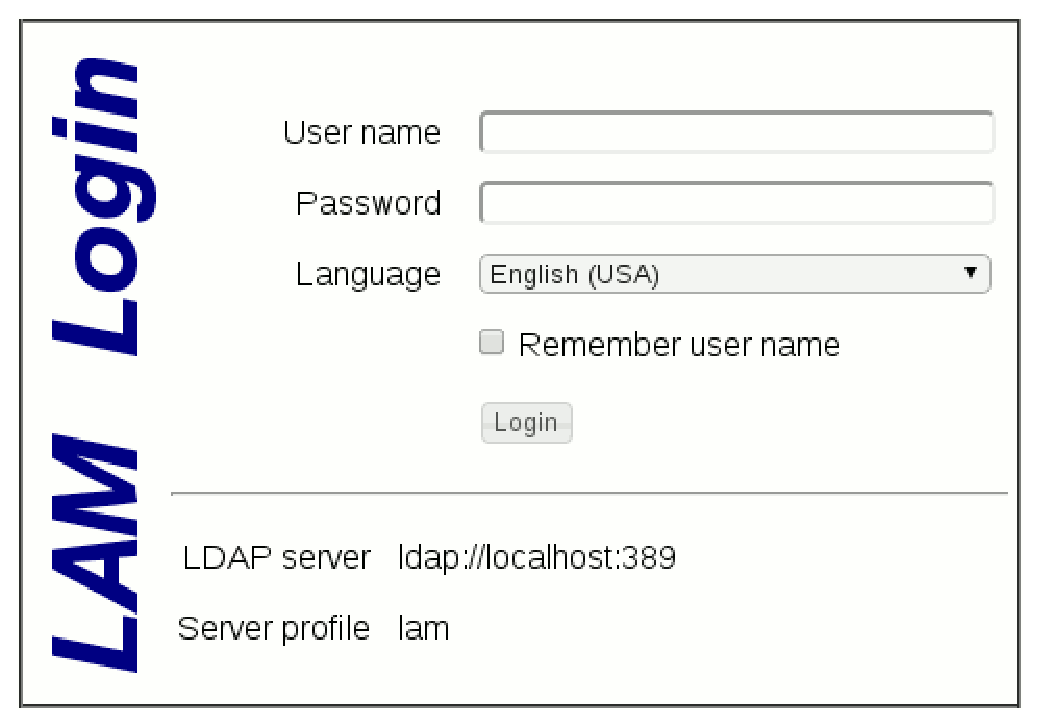
\includegraphics[scale=0.4,keepaspectratio=true]{figures/LAM}

\end{frame}

%------------------------------------------------

\begin{frame}
\frametitle{Desarrollo}
\framesubtitle{Interfaz de cambio de contrase\~{n}a}

LDAP Toolbox - Self Service Password

\vspace{1em}

\centering
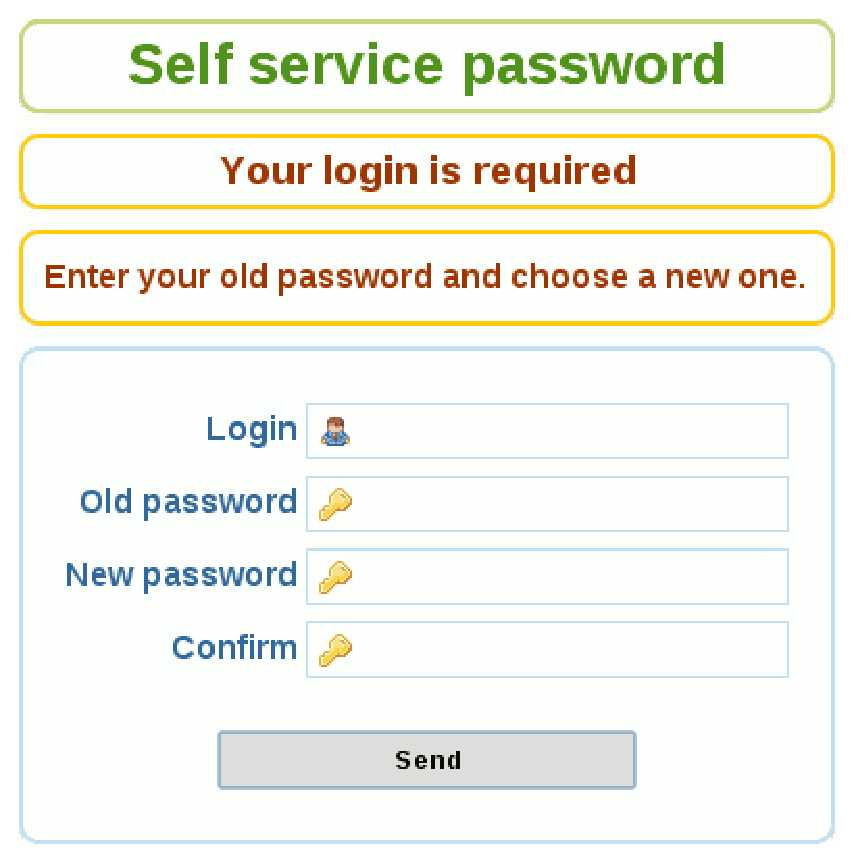
\includegraphics[scale=0.4,keepaspectratio=true]{figures/Self-Service-Password}

\end{frame}

%------------------------------------------------

\begin{frame}
\frametitle{Desarrollo}
\framesubtitle{\textsl{Hardening}}
\justifying
\begin{itemize}
 \item Actualizaciones desatendidas
\\~\\
 \item Reducci\'{o}n de componentes instalados
\\~\\
 \item Configuraci\'{o}n de seguridad de \textup{OpenSSH}
\\~\\
 \item Configuraci\'{o}n de seguridad de Apache \textup{HTTPD} y \textup{PHP}
\\~\\
 \item Par\'{a}metros de cifrado para \textup{HTTPS}
\\~\\
 \item Reglas de \textsl{Firewall}
\end{itemize}

\end{frame}

%------------------------------------------------

\begin{frame}
\frametitle{Pruebas}
\justifying

\begin{block}{\textbf{Compatibilidad multiplataforma}}
 \begin{itemize}
  \item Sistemas operativos de escritorio y m\'{o}viles
  \item Navegadores web
 \end{itemize}
\end{block}

% The "c" option specifies centered vertical alignment while the "t" option is used for top vertical alignment
\begin{columns}[c] 

\column{.45\textwidth}
\begin{block}{\textbf{Roles de usuario}}
 \begin{itemize}
  \item S\'{o}lo lectura
  \item Lectura / Escritura
 \end{itemize}
\end{block}

\column{.45\textwidth}
\begin{block}{\textbf{Seguridad}}
 \begin{itemize}
  \item Puertos abiertos
  \item Par\'{a}metros de cifrado para \textup{HTTPS}
 \end{itemize}
\end{block}

\end{columns}

\end{frame}

%%------------------------------------------------
%
% \begin{frame}
% \frametitle{Problemas encontrados}
% \justifying
% 
% \textbf{\textup{WebDAV}}
% \begin{itemize}
%  \item El soporte en clientes Windows es bastante limitado
%  \item Es necesario deshabilitar la auto-detecci\'{o}n de proxy
% \end{itemize}
% 
% \textbf{\textup{HTTPS}}
% \begin{itemize}
%  \item Es necesario distribuir el certificado ra\'{i}z de la autoridad certificadora
%  \item Requisito para la conexi\'{o}n en clientes Windows
% \end{itemize}
%
% \textbf{\textup{LDAP}}
% \begin{itemize}
%  \item La carga correcta de usuarios requiere validar muchos campos
%  \item Los archivos de entrada no son del todo confiables o veraces
% \end{itemize}
% 
% \end{frame}

%------------------------------------------------

\begin{frame}
\frametitle{Conclusiones}
\framesubtitle{Resultados obtenidos}
\justifying

\textbf{\textup{WebDAV}}
\begin{itemize}
 \item Compatibilidad
 \item Integraci\'{o}n con otras plataformas
\end{itemize}

\vspace{2em}

\textbf{\textup{HTTPS}}
\begin{itemize}
 \item Proteje la confidencialidad e integridad de la informaci\'{o}n
 \item Requisito para la conexi\'{o}n en clientes Windows
\end{itemize}

\end{frame}

%------------------------------------------------

\begin{frame}
\frametitle{Conclusiones}
\framesubtitle{Resultados obtenidos}
\justifying

\textbf{Compatibilidad multiplataforma}
\begin{itemize}
 \item Ajustes para compatibilidad con clientes Windows
 \item Instalaci\'{o}n del certificado ra\'{i}z en los clientes
\end{itemize}

\vspace{2em}

\textbf{Autenticaci\'{o}n \textup{LDAP}}
\begin{itemize}
 \item Carga de usuarios desde archivos \textup{CSV}
 \item Se puede hacer la carga de forma parcial o completa
\end{itemize}

\end{frame}

%------------------------------------------------

\begin{frame}
\frametitle{Conclusiones}
\framesubtitle{Oportunidades de mejora}
\justifying

\textbf{Cuotas de disco duro}
\begin{itemize}
 \item Limita el espacio de disco disponible a cada usuario
 \item Requiere el uso de ACL en el sistema de archivos
\end{itemize}

\vspace{2em}

\textbf{Otros mecanismos de autenticaci\'{o}n}
\begin{itemize}
 \item Conexi\'{o}n con otros directorios \textup{LDAP} y bases de datos \textup{SQL}
 \item Requiere modificaciones a los filtros de b\'{u}squeda
\end{itemize}

\end{frame}

%------------------------------------------------

\begin{frame}
\frametitle{Conclusiones}
\framesubtitle{Oportunidades de mejora}
\justifying

\textbf{Autenticaci\'{o}n \textup{LDAP}}
\begin{itemize}
 \item El directorio puede autenticar usuarios de otros sistemas
 \item Requiere grupos adicionales para el manejo de privilegios
\end{itemize}

\vspace{2em}

\textbf{Integraci\'{o}n con \textsl{ownCloud}}
\begin{itemize}
 \item Puede ser utilizado como fuente de autenticaci\'{o}n
\\~\\
% \item Es posible montar el directorio virtual de \textup{xNAS} en \textup{ownCloud}
\end{itemize}

\end{frame}

%------------------------------------------------

\begin{frame}
\centering
 \psscalebox{2.5 2.5}
 {
  \begin{pspicture}(0,-0.295)(2.63,0.295)
   \rput[bl](0.75,-0.6){\Huge{\Thanks}}
  \end{pspicture}
 }
\end{frame}

%------------------------------------------------

\end{document}

